\section{Casos de uso}

\subsection{Actores del sistema}

Tras las reuniones con los clientes, se determinaron los perfiles de personas que iban a utilizar el sistema y se plasmaron en los requisitos. Estos usarán el sistema en forma de usuarios y representados por diferentes roles.

Dentro que se han determinado las posibles acciones dentro de cada rol, para clarificar cada tipo de usuario, se definirán estos como los actores que hacen uso del sistema. A parte de estos, no se consideran otros actores externos de forma relevante para explicarlos en forma de tabla. Son los siguientes: 

\begin{table}[H]
    \centering
    \resizebox{\textwidth}{!}{%
        \begin{tabular}{|l|l|l|} 
        \hline
        \rowcolor[rgb]{0.886,0.886,0.886} \textbf{Actor}            & Usuario administrador                                                                                              & \multicolumn{1}{c|}{ACT\_1}                   \\ 
        \hline
        \textbf{Descripción}                                        & \multicolumn{2}{l|}{Usuario con los máximos privilegios posibles en el sistema.}                                                                                   \\ 
        \hline
        \textbf{Características}                                    & \multicolumn{2}{l|}{\begin{tabular}[c]{@{}l@{}}Está destinado principalmente a la gente que gestiona\\ la fundación y supervisa el trabajo de otros\end{tabular}}  \\ 
        \hline
        \textbf{Relaciones}                                         & \multicolumn{2}{l|}{}                                                                                                                                              \\ 
        \hline
        \textbf{Referencias}                                        & \multicolumn{2}{l|}{\textit{(Añadir elementos en los que interviene)}}                                                                                             \\ 
        \hline
        \multicolumn{3}{l}{}                                                                                                                                                                                                             \\ 
        \hline
        \multicolumn{3}{|l|}{{\cellcolor[rgb]{0.886,0.886,0.886}}\textbf{Atributos}}                                                                                                                                                     \\ 
        \hline
        \textbf{Nombre}                                             & \textbf{Descripción}                                                                                               & \textbf{Tipo}                                 \\ 
        \hline
        Persona asociada                                            & \begin{tabular}[c]{@{}l@{}}Se almacenará la persona asociada en caso de\\que se quiera asociar alguna\end{tabular} & Persona                                       \\ 
        \hline
        Nombre                                                      & Nombre de la persona                                                                                               & String                                        \\ 
        \hline
        Contraseña                                                  & Contraseña del usuario                                                                                             & String                                        \\ 
        \hline
        \begin{tabular}[c]{@{}l@{}}Nombre de \\usuario\end{tabular} & \begin{tabular}[c]{@{}l@{}}Nombre de usuario identificativo utilizado para\\iniciar sesión\end{tabular}            & String                                        \\ 
        \hline
        \end{tabular}
    }
    \caption{Descripción del usuario administrador}
\end{table}

\begin{table}[H]
    \centering
    \resizebox{\textwidth}{!}{%
        \begin{tabular}{|l|l|l|} 
        \hline
        \rowcolor[rgb]{0.886,0.886,0.886} \textbf{Actor} & Usuario general & ACT\_2                                                                                                                                        \\ 
        \hline
        \textbf{Descripción}                             & \multicolumn{2}{l|}{\begin{tabular}[c]{@{}l@{}}Usuario con privilegios de edición pero no sobre acciones~~~ \\críticas\end{tabular}}                            \\ 
        \hline
        \textbf{Características}                         & \multicolumn{2}{l|}{\begin{tabular}[c]{@{}l@{}}Está destinado a gente que colabore con la fundación pero \\con limitaciones en acciones críticas\end{tabular}}  \\ 
        \hline
        \textbf{Relaciones}                              & \multicolumn{2}{l|}{}                                                                                                                                           \\ 
        \hline
        \textbf{Referencias}                             & \multicolumn{2}{l|}{\textit{(Añadir elementos en los que interviene)}}                                                                                          \\
        \hline
        \multicolumn{3}{l}{}                                                                                                                                                                                                             \\ 
        \hline
        \multicolumn{3}{|l|}{{\cellcolor[rgb]{0.886,0.886,0.886}}\textbf{Atributos}}                                                                                                                                                     \\ 
        \hline
        \textbf{Nombre}                                             & \textbf{Descripción}                                                                                               & \textbf{Tipo}                                 \\ 
        \hline
        Persona asociada                                            & \begin{tabular}[c]{@{}l@{}}Se almacenará la persona asociada en caso de\\que se quiera asociar alguna\end{tabular} & Persona                                       \\ 
        \hline
        Nombre                                                      & Nombre de la persona                                                                                               & String                                        \\ 
        \hline
        Contraseña                                                  & Contraseña del usuario                                                                                             & String                                        \\ 
        \hline
        \begin{tabular}[c]{@{}l@{}}Nombre de \\usuario\end{tabular} & \begin{tabular}[c]{@{}l@{}}Nombre de usuario identificativo utilizado para\\iniciar sesión\end{tabular}            & String                                        \\ 
        \hline
        \end{tabular}
    }
    \caption{Descripción del usuario general}
\end{table}

\begin{table}[H]
    \centering
    \resizebox{\textwidth}{!}{
        \begin{tabular}{|l|l|c|} 
            \hline
            \rowcolor[rgb]{0.886,0.886,0.886} \textbf{Actor}            & Usuario participante                                                                                                                                             & ACT\_4         \\ 
            \hline
            \textbf{Descripción}                                        & \multicolumn{2}{l|}{\begin{tabular}[c]{@{}l@{}}Usuario con privilegios de acceso solo a la sección de \\actividades\end{tabular}}                                                 \\ 
            \hline
            \textbf{Características}                                    & \multicolumn{2}{l|}{\begin{tabular}[c]{@{}l@{}}Está destinado a residentes de la fundación que participan\\en los talleres realizados por esta.\end{tabular}}                     \\ 
            \hline
            \textbf{Relaciones}                                         & \multicolumn{2}{l|}{}                                                                                                                                                             \\ 
            \hline
            \textbf{Referencias}                                        & \multicolumn{2}{l|}{\textit{(Añadir elementos en los que interviene)}}                                                                                                            \\ 
            \hline
            \multicolumn{3}{l}{}                                                                                                                                                                                                                            \\ 
            \hline
            \multicolumn{3}{|l|}{{\cellcolor[rgb]{0.886,0.886,0.886}}\textbf{Atributos}}                                                                                                                                                                    \\ 
            \hline
            \textbf{Nombre}                                             & \textbf{Descripción}                                                                                                                                             & \textbf{Tipo}  \\ 
            \hline
            Persona asociada                                            & \begin{tabular}[c]{@{}l@{}}Se almacenará la persona asociada. Esta será\\estrictamente necesaria en caso de que se \\quiera apuntar en actividades.\end{tabular} & Persona        \\ 
            \hline
            Nombre                                                      & Nombre de la persona                                                                                                                                             & String         \\ 
            \hline
            Contraseña                                                  & Contraseña del usuario                                                                                                                                           & String         \\ 
            \hline
            \begin{tabular}[c]{@{}l@{}}Nombre de \\usuario\end{tabular} & \begin{tabular}[c]{@{}l@{}}Nombre de usuario identificativo utilizado para\\iniciar sesión\end{tabular}                                                          & String         \\
            \hline
        \end{tabular}
    }
    \caption{Descripción del usuario participante}
\end{table}

\begin{table}[H]
    \centering
    \resizebox{\textwidth}{!}{%
        \begin{tabular}{|l|l|l|} 
            \hline
            \rowcolor[rgb]{0.886,0.886,0.886} \textbf{Actor}             & Usuario invitado                                                                                                                                            & ACT\_3                                                                   \\ 
            \hline
            \textbf{Descripción}                                         & \multicolumn{2}{l|}{\begin{tabular}[c]{@{}l@{}}Usuario con privilegios de acceso a la información y no de \\edición con limitaciones opcionales a diferentes secciones.\end{tabular}}                                                  \\ 
            \hline
            \textbf{Características}                                     & \multicolumn{2}{l|}{\begin{tabular}[c]{@{}l@{}}Está destinado a gente con la que la fundación trabaje. \\Sin ser parte de esta, puede existir cierta gente a la que\\la fundación tenga interés de mostrar información.\end{tabular}}  \\ 
            \hline
            \textbf{Relaciones}                                          & \multicolumn{2}{l|}{}                                                                                                                                                                                                                  \\ 
            \hline
            \textbf{Referencias}                                         & \multicolumn{2}{l|}{\textit{(Añadir elementos en los que interviene)}}                                                                                                                                                                 \\ 
            \hline
            \multicolumn{3}{l}{}                                                                                                                                                                                                                                                                                  \\ 
            \hline
            \multicolumn{3}{|l|}{{\cellcolor[rgb]{0.886,0.886,0.886}}\textbf{Atributos}}                                                                                                                                                                                                                          \\ 
            \hline
            \textbf{Nombre}                                              & \textbf{Descripción}                                                                                                                                        & \textbf{Tipo}                                                            \\ 
            \hline
            Persona asociada                                             & \begin{tabular}[c]{@{}l@{}}Se almacenará la persona asociada en caso de\\que se quiera asociar alguna\end{tabular}                                          & Persona                                                                  \\ 
            \hline
            Nombre                                                       & Nombre de la persona                                                                                                                                        & String                                                                   \\ 
            \hline
            Contraseña                                                   & Contraseña del usuario                                                                                                                                      & String                                                                   \\ 
            \hline
            \begin{tabular}[c]{@{}l@{}}Nombre de \\usuario\end{tabular}  & \begin{tabular}[c]{@{}l@{}}Nombre de usuario identificativo utilizado para\\iniciar sesión\end{tabular}                                                     & String                                                                   \\ 
            \hline
            \begin{tabular}[c]{@{}l@{}}Permisos de \\acceso\end{tabular} & \begin{tabular}[c]{@{}l@{}}Permisos de acceso a diferentes sesiones o \\tipos de personas que restringirán las \\posibilidades de este usuario\end{tabular} & \multicolumn{1}{l|}{Booleanos}                                           \\ 
            \hline
            \multicolumn{3}{l}{}                                                                                                                                                                                                                                                                                  \\ 
            \hline
            \multicolumn{3}{|l|}{{\cellcolor[rgb]{0.886,0.886,0.886}}\textbf{Comentarios}}                                                                                                                                                                                                                        \\ 
            \hline
            \multicolumn{3}{|l|}{\begin{tabular}[c]{@{}l@{}}Este usuario podrá tener limitado el acceso por secciones y por tipos de\\personas.\end{tabular}}                                                                                                                                                     \\
            \hline
        \end{tabular}
    }
    \caption{Descripción del usuario invitado}
\end{table}

\subsection{Usuarios}

El sistema estará planteado de forma que solo el usuario administrador pueda gestionar los usuarios del sistema. Es por esto, que este tipo de usuarios estén dirigidos a personas con un mayor nivel de responsabilidad en la fundación. El resto de usuarios, solo podrán loguearse en el sistema, es decir, solicitar permisos de acceso a este para poder acceder a los recursos pertinentes y desloguearse, buscando que el sistema invalide los mecanismos de acceso a la información para este usuario.

El diagrama de casos de uso que representa estas acciones viene representado en la Figura \ref{fig:cu_usuarios}. En esta se puede ver como el actor referente a los usuarios administradores gestionan a los usuarios, mientras que todos los demás solo tienen acceso a métodos de login y logout. 

\begin{figure}[hp!]
    \centering
    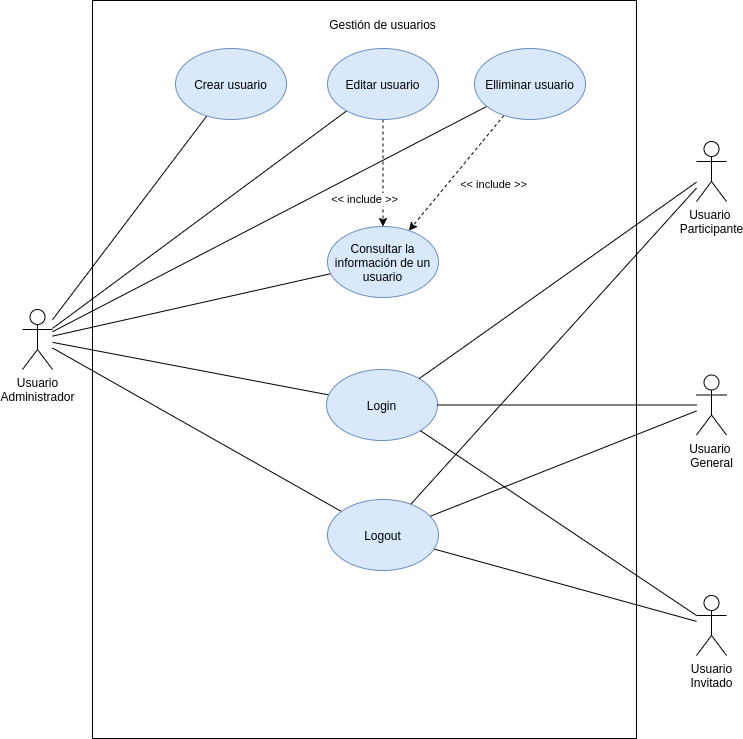
\includegraphics[width=1\linewidth]{diseno/sistema/CU/usuarios.png}
    \caption{Diagrama de casos de uso referente a la gestión de usuarios}
    \label{fig:cu_usuarios}
\end{figure}

Dentro de la gestión de usuarios, el caso de uso a destacar, por tener un flujo de funcionamiento diferente a los demás y alejado de operaciones simples sobre datos, será el de login. Para entender mejor la idea de este, se ha desarrollado una descripción este en la Tabla \ref{fig:cu_usuarios_login}.

\begin{table}[hp!]
    \centering
    \resizebox{\textwidth}{!}{
        \begin{tabular}{|l|l|l|l|} 
        \hline
        \rowcolor[rgb]{0.886,0.886,0.886} \textbf{Caso de uso} & \multicolumn{2}{l|}{Login}              & CU\_01                                                                                                                                        \\ 
        \hline
        \textbf{Actores}                                       & \multicolumn{3}{l|}{ACT\_1, ACT\_2, ACT\_3, ACT\_4}                                                                                                                                     \\ 
        \hline
        \textbf{Tipo}                                          & \multicolumn{3}{l|}{Primario}                                                                                                                                                           \\ 
        \hline
        \textbf{Referencias}                                   &                      & \multicolumn{2}{l|}{}                                                                                                                                            \\ 
        \hline
        \textbf{Precondición}                                  & \multicolumn{3}{l|}{Conocer el nombre de usuario y la contraseña}                                                                                                                       \\ 
        \hline
        \textbf{Poscondición}                                  & \multicolumn{3}{l|}{\begin{tabular}[c]{@{}l@{}}El usuario podrá acceder a los recursos del sistema sobre \\los que tiene permisos.\end{tabular}}                                        \\ 
        \hline
        \textbf{Autor}                                         & Pablo Cordero Romero & \textbf{Versión} & 1.0                                                                                                                                           \\ 
        \hline
        \multicolumn{4}{l}{}                                                                                                                                                                                                                             \\ 
        \hline
        \multicolumn{4}{|l|}{{\cellcolor[rgb]{0.886,0.886,0.886}}\textbf{Propósito}}                                                                                                                                                                     \\ 
        \hline
        \multicolumn{4}{|l|}{\begin{tabular}[c]{@{}l@{}}Permitir a un usuario acceder al sistema con su contraseña y nombre de\\usuario\end{tabular}}                                                                                                    \\ 
        \hline
        \multicolumn{4}{l}{}                                                                                                                                                                                                                             \\ 
        \hline
        \multicolumn{4}{|l|}{{\cellcolor[rgb]{0.886,0.886,0.886}}\textbf{Resumen}}                                                                                                                                                                       \\ 
        \hline
        \multicolumn{4}{|l|}{\begin{tabular}[c]{@{}l@{}}Un usuario, indicando su nombre usuario y contraseña, obtiene un\\mecanismo de autenticación que le permite acceder a los recursos del \\sistema sobre los que tiene permisos. \end{tabular}}    \\
        \hline
        \end{tabular}
    }
    \caption{Caso de uso 1: Login}
    \label{fig:cu_usuarios_login}
\end{table}


\begin{table}[hp!]
    \centering
    \resizebox{\textwidth}{!}{
        \begin{tabular}{|l|l|l|l|} 
        \hline
        \multicolumn{4}{|l|}{{\cellcolor[rgb]{0.886,0.886,0.886}}\textbf{Curso Normal (básico) de eventos}}                                                                                                                                   \\ 
        \hline
        \multicolumn{2}{|l|}{\textit{\textbf{Actor}}}                                                             & \multicolumn{2}{l|}{\textit{\textbf{Sistema}}}                                                                            \\ 
        \hline
        1  & \begin{tabular}[c]{@{}l@{}}El usuario envía su usuario y\\contraseña\end{tabular}                    & 2 & \begin{tabular}[c]{@{}l@{}}El sistema comprueba que el usuario \\existe y que la contraseña es correcta\end{tabular}  \\ 
        \hline
        &                                                                                                      & 3 & \begin{tabular}[c]{@{}l@{}}El sistema envía un método de\\identificación al usuario\end{tabular}                      \\ 
        \hline
        4  & \begin{tabular}[c]{@{}l@{}}El usuario recibe el método de\\identificación y lo almacena\end{tabular} &   &                                                                                                                       \\ 
        \hline
        \multicolumn{4}{l}{}                                                                                                                                                                                                                  \\ 
        \hline
        \multicolumn{4}{|l|}{{\cellcolor[rgb]{0.886,0.886,0.886}}\textbf{Curso Alterno (secundario) de eventos}}                                                                                                                              \\ 
        \hline
        3a & \multicolumn{3}{l|}{ El usuario no existe en el sistema o la contraseña es incorrecta }                                                                                                                                          \\ 
        \hline
        & \multicolumn{3}{l|}{1. El sistema notifica al usuario de que el acceso es incorrecto}                                                                                                                                            \\
        \hline
        \end{tabular}
    }
    \caption{Curso de eventos del caso de uso 1}
\end{table}

\newpage

\subsection{Personas}

En la gestión de todo lo referente a las personas, habrá mas operaciones. En este, no solo el usuario administrador tendrá el protagonismo, sin no que también participarán los usuarios generales e invitados si tienen los respectivos permisos.

Aquí no solo entran los datos directos de las personas, si no también la gestión de sus documentos, citas, y su estado actual, si es de alta o de baja. El diagrama de casos de uso referente a esta sección está representado en la Figura \ref{fig:cu_personas}. 

\begin{figure}[h!]
    \centering
    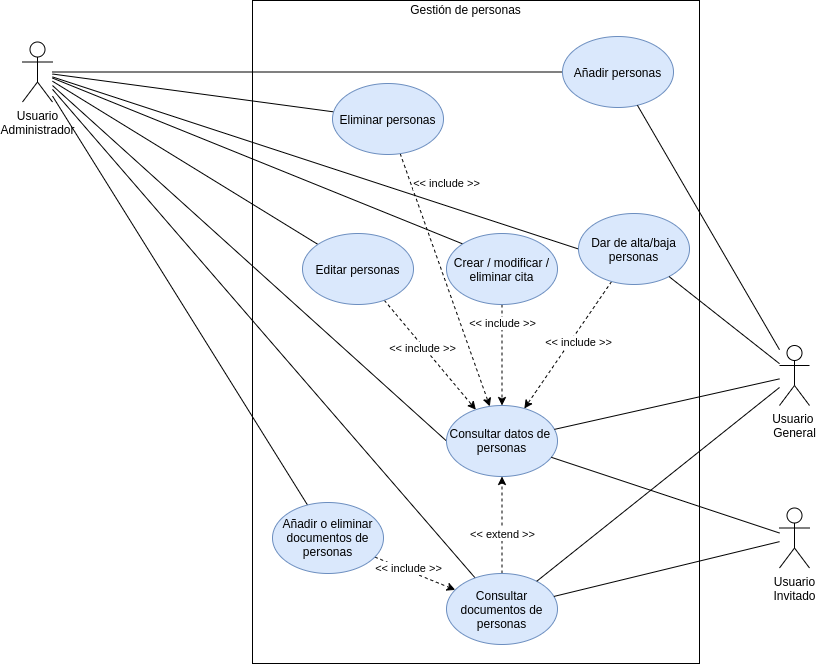
\includegraphics[width=1\linewidth]{diseno/sistema/CU/personas.png}
    \caption{Diagrama de casos de uso referente a la gestión de personas}
    \label{fig:cu_personas}
\end{figure}

Dentro de los casos de usos representados, el que más dudas puede generar será el de dar de alta o de baja a las personas. El dar de baja es algo confuso, y puede verse relacionado con el eliminar una personas del sistema. Las plantillas de estos casos de uso (Tablas \ref{fig:cu_personas_altabaja} y \ref{fig:cu_personas_eliminar}) clarifican el funcionamiento que se busca en estos.

\begin{table}[hp!]
    \centering
    \resizebox{\textwidth}{!}{
        \begin{tabular}{|l|l|l|l|} 
        \hline
        \rowcolor[rgb]{0.886,0.886,0.886} \textbf{Caso de uso} & \multicolumn{2}{l|}{Eliminar persona}   & CU\_02                                                                                                      \\ 
        \hline
        \textbf{Actores}                                       & \multicolumn{3}{l|}{ACT\_1\textit{}}                                                                                                                  \\ 
        \hline
        \textbf{Tipo}                                          & \multicolumn{3}{l|}{Primario}                                                                                                                         \\ 
        \hline
        \textbf{Referencias}                                   &                      & \multicolumn{2}{l|}{}                                                                                                          \\ 
        \hline
        \textbf{Precondición}                                  & \multicolumn{3}{l|}{Se conoce la información de la persona}                                                                                           \\ 
        \hline
        \textbf{Poscondición}                                  & \multicolumn{3}{l|}{Toda la información de la persona es eliminada del sistema}                                                                       \\ 
        \hline
        \textbf{Autor}                                         & Pablo Cordero Romero & \textbf{Versión} & 1.0                                                                                                         \\ 
        \hline
        \multicolumn{4}{l}{}                                                                                                                                                                                           \\ 
        \hline
        \multicolumn{4}{|l|}{{\cellcolor[rgb]{0.886,0.886,0.886}}\textbf{Propósito}}                                                                                                                                   \\ 
        \hline
        \multicolumn{4}{|l|}{Eliminar la información de un persona del sistema}                                                                                                                                        \\ 
        \hline
        \multicolumn{4}{l}{}                                                                                                                                                                                           \\ 
        \hline
        \multicolumn{4}{|l|}{{\cellcolor[rgb]{0.886,0.886,0.886}}\textbf{Resumen}}                                                                                                                                     \\ 
        \hline
        \multicolumn{4}{|l|}{\begin{tabular}[c]{@{}l@{}}Al eliminar una persona del sistema, todas la información directa de esta\\e indirecta (alojamiento, citas) dejará de ser almacenada en este.\end{tabular}}    \\
        \hline
        \end{tabular}
    }
    \caption{Caso de uso 2: Eliminar una persona}
    \label{fig:cu_personas_eliminar}
\end{table}

\begin{table}[hp!]
    \centering
    \resizebox{\textwidth}{!}{
        \begin{tabular}{|l|l|l|l|} 
        \hline
        \multicolumn{4}{|l|}{{\cellcolor[rgb]{0.886,0.886,0.886}}\textbf{Curso Normal (básico) de eventos}}                                                                                                                                                                                             \\ 
        \hline
        \multicolumn{2}{|l|}{\textit{\textbf{Actor}}}                                                                         & \multicolumn{2}{l|}{\textit{\textbf{Sistema}}}                                                                                                                          \\ 
        \hline
        1  & \begin{tabular}[c]{@{}l@{}}El usuario solicita eliminar una\\persona del sistema\end{tabular}                    & 2 & \begin{tabular}[c]{@{}l@{}}El sistema comprueba que la persona\\existe en el sistema.\end{tabular}                                                                  \\ 
        \hline
        &                                                                                                                  & 3 & \begin{tabular}[c]{@{}l@{}}El sistema elimina al completo toda la\\información relacionada con la persona\\(documentos, fotografías, datos, citas...)\end{tabular}  \\ 
        \hline
        4  & \begin{tabular}[c]{@{}l@{}}El usuario recibe la confirmación\\de que se ha realizado\\correctamente\end{tabular} &   &                                                                                                                                                                     \\ 
        \hline
        \multicolumn{4}{l}{}                                                                                                                                                                                                                                                                            \\ 
        \hline
        \multicolumn{4}{|l|}{{\cellcolor[rgb]{0.886,0.886,0.886}}\textbf{Curso Alterno (secundario) de eventos}}                                                                                                                                                                                        \\ 
        \hline
        3a & \multicolumn{3}{l|}{La persona no existe en el sistema}                                                                                                                                                                                                                                    \\ 
        \hline
        & \multicolumn{3}{l|}{1. El sistema notifica al usuario de que la persona no existe}                                                                                                                                                                                                         \\ 
        \hline
        \multicolumn{4}{l}{}                                                                                                                                                                                                                                                                            \\ 
        \hline
        \multicolumn{4}{|l|}{{\cellcolor[rgb]{0.886,0.886,0.886}}\textbf{Comentarios}}                                                                                                                                                                                                                  \\ 
        \hline
        \multicolumn{4}{|l|}{Se eliminará cualquier registro existente de la persona en el sistema}                                                                                                                                                                                                     \\
        \hline
        \end{tabular}
    }
    \caption{Curso de eventos del caso de uso 2}
\end{table}

\begin{table}[hp!]
    \centering
    \resizebox{\textwidth}{!}{
        \begin{tabular}{|l|l|l|l|} 
        \hline
        \rowcolor[rgb]{0.886,0.886,0.886} \textbf{Caso de uso} & \multicolumn{2}{l|}{Dar de alta/baja una persona} & CU\_03                                                                                                                                                                                                                         \\ 
        \hline
        \textbf{Actores}                                       & \multicolumn{3}{l|}{ACT\_1, ACT\_2\textit{}}                                                                                                                                                                                                                                       \\ 
        \hline
        \textbf{Tipo}                                          & \multicolumn{3}{l|}{Secundario}                                                                                                                                                                                                                                                    \\ 
        \hline
        \textbf{Referencias}                                   &                      & \multicolumn{2}{l|}{}                                                                                                                                                                                                                                       \\ 
        \hline
        \textbf{Precondición}                                  & \multicolumn{3}{l|}{\begin{tabular}[c]{@{}l@{}}Se conoce la información del usuario junto con si está\\actualmente dado de baja o del alta\end{tabular}}                                                                                                                           \\ 
        \hline
        \textbf{Poscondición}                                  & \multicolumn{3}{l|}{\begin{tabular}[c]{@{}l@{}}El estado de la persona en cuestión cambiará. Si la\\persona es dada de baja, en caso de que forme parte\\de una habitación, el puesto de alojamiento será\\liberado.\\\end{tabular}}                                               \\ 
        \hline
        \textbf{Autor}                                         & Pablo Cordero Romero & \textbf{Versión}           & 1.0                                                                                                                                                                                                                            \\ 
        \hline
        \multicolumn{4}{l}{}                                                                                                                                                                                                                                                                                                                        \\ 
        \hline
        \multicolumn{4}{|l|}{{\cellcolor[rgb]{0.886,0.886,0.886}}\textbf{Propósito}}                                                                                                                                                                                                                                                                \\ 
        \hline
        \multicolumn{4}{|l|}{Cambiar el estado de una persona}                                                                                                                                                                                                                                                                                      \\ 
        \hline
        \multicolumn{4}{l}{}                                                                                                                                                                                                                                                                                                                        \\ 
        \hline
        \multicolumn{4}{|l|}{{\cellcolor[rgb]{0.886,0.886,0.886}}\textbf{Resumen}}                                                                                                                                                                                                                                                                  \\ 
        \hline
        \multicolumn{4}{|l|}{\begin{tabular}[c]{@{}l@{}}Al cambiar el estado de una persona, esta pasará a estar de alta, si\\entra en la fundación de alguna forma, y de baja si ya no está \\relacionado directamente con esta. Esto sirve de igual forma tanto \\para residentes como para voluntarios, socios y colaboradores.\end{tabular}}    \\
        \hline
        \end{tabular}
    }
    \caption{Caso de uso 3: Dar de alta/baja una persona}
    \label{fig:cu_personas_altabaja}
\end{table}

\begin{table}[hp!]
    \centering
    \resizebox{\textwidth}{!}{
        \begin{tabular}{|l|l|l|l|} 
        \hline
        \multicolumn{4}{|l|}{{\cellcolor[rgb]{0.886,0.886,0.886}}\textbf{Curso Normal (básico) de eventos}}                                                                                                                                                                                               \\ 
        \hline
        \multicolumn{2}{|l|}{\textit{\textbf{Actor}}}                                                                         & \multicolumn{2}{l|}{\textit{\textbf{Sistema}}}                                                                                                                            \\ 
        \hline
        1  & \begin{tabular}[c]{@{}l@{}}El usuario solicita dar de alta~~~~ \\o baja a una persona\end{tabular}               & 2 & \begin{tabular}[c]{@{}l@{}}El sistema comprueba que la persona no\\tenga ya el estado que se le quiere dar\end{tabular}                                               \\ 
        \hline
        &                                                                                                                  & 3 & \begin{tabular}[c]{@{}l@{}}El sistema da de baja/alta a la persona\\eliminando únicamente su plaza de\\alojamiento\end{tabular}                                       \\ 
        \hline
        4  & \begin{tabular}[c]{@{}l@{}}El usuario recibe la confirmación\\de que se ha realizado\\correctamente\end{tabular} &   &                                                                                                                                                                       \\ 
        \hline
        \multicolumn{4}{l}{}                                                                                                                                                                                                                                                                              \\ 
        \hline
        \multicolumn{4}{|l|}{{\cellcolor[rgb]{0.886,0.886,0.886}}\textbf{Curso Alterno (secundario) de eventos}}                                                                                                                                                                                          \\ 
        \hline
        3a & \multicolumn{3}{l|}{La persona no existe en el sistema}                                                                                                                                                                                                                                      \\ 
        \hline
        & \multicolumn{3}{l|}{1. El sistema notifica al usuario de que la persona no existe}                                                                                                                                                                                                           \\ 
        \hline
        3b & \multicolumn{3}{l|}{La persona que se intenta dar de alta, actualmente está dada de alta}                                                                                                                                                                                                    \\ 
        \hline
        & \multicolumn{3}{l|}{1. El sistema notifica al usuario que la persona ya está dada de alta}                                                                                                                                                                                                   \\ 
        \hline
        3c & \multicolumn{3}{l|}{La persona que se intenta dar de baja, actualmente está dada de baja}                                                                                                                                                                                                    \\ 
        \hline
        & \multicolumn{3}{l|}{1. El sistema notifica al usuarios que la persona ya está dada de baja}                                                                                                                                                                                                  \\ 
        \hline
        \multicolumn{4}{l}{}                                                                                                                                                                                                                                                                              \\ 
        \hline
        \multicolumn{4}{|l|}{{\cellcolor[rgb]{0.886,0.886,0.886}}\textbf{Comentarios}}                                                                                                                                                                                                                    \\ 
        \hline
        \multicolumn{4}{|l|}{\begin{tabular}[c]{@{}l@{}}La persona no aparecerá como persona activa, pero sus datos permanecerán en\\el sistema almacenados. En caso de ser un residente, su plaza de alojamiento\\quedará vacía ya que se considerará que ya no reside en la fundación.\end{tabular}}    \\
        \hline
        \end{tabular}
    }
    \caption{Curso de eventos del caso de uso 3}
\end{table}

\newpage

\subsection{Alojamientos}

En la gestión de alojamientos, ocurre como con la gestión de personas, participan los usuarios con el rol de administrador, invitado y general. Esta gestión consistirá principalmente en la gestión de las propiedades del alojamiento junto con los residentes de cada una de las habitaciones. 

Dentro de los casos de usos mostrados en el diagrama de casos de uso de la Figura \ref{fig:cu_alojamientos}, los más difíciles de entender pueden ser los referidos a la modificación de una habitación. Con el objetivo de explicar un poco mejor el funcionamiento de ambos, se han realizado la descripción correspondiente de cada uno de ellos en las tablas \ref{fig:cu_alojamientos_modificar} y \ref{fig:cu_alojamientos_modificarresidentes}. 

\begin{figure}[h!]
    \centering
    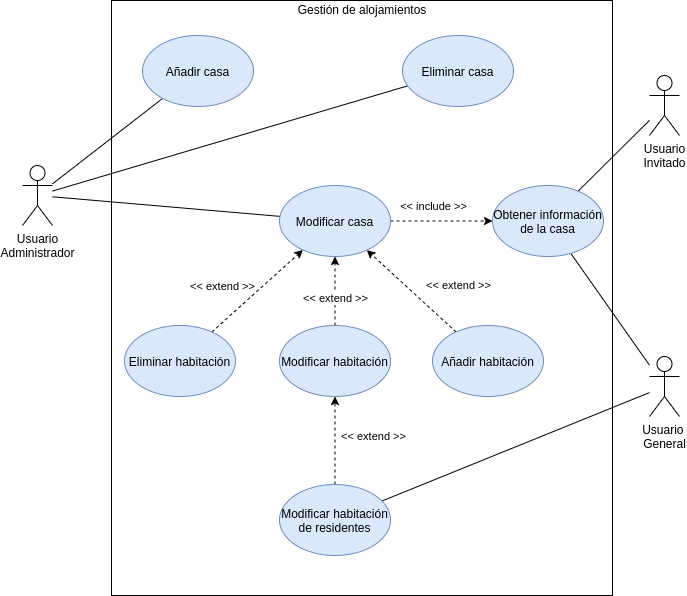
\includegraphics[width=1\linewidth]{diseno/sistema/CU/alojamiento.png}
    \caption{Diagrama de casos de uso referente a la gestión de alojamientos}
    \label{fig:cu_alojamientos}
\end{figure}

\begin{table}[hp!]
    \centering
    \resizebox{\textwidth}{!}{
        \begin{tabular}{|l|l|l|l|} 
        \hline
        \rowcolor[rgb]{0.886,0.886,0.886} \textbf{Caso de uso} & \multicolumn{2}{l|}{Modificar habitación} & CU\_04                                                                  \\ 
        \hline
        \textbf{Actores}                                       & \multicolumn{3}{l|}{ACT\_1}                                                                                         \\ 
        \hline
        \textbf{Tipo}                                          & \multicolumn{3}{l|}{Primario}                                                                                       \\ 
        \hline
        \textbf{Referencias}                                   &                      & \multicolumn{2}{l|}{}                                                                        \\ 
        \hline
        \textbf{Precondición}                                  & \multicolumn{3}{l|}{Se está modificando la casa}                                                                    \\ 
        \hline
        \textbf{Poscondición}                                  & \multicolumn{3}{l|}{La información de la habitación es modificada (junto con los residentes)}                       \\ 
        \hline
        \textbf{Autor}                                         & Pablo Cordero Romero & \textbf{Versión}   & 1.0                                                                     \\ 
        \hline
        \multicolumn{4}{l}{}                                                                                                                                                         \\ 
        \hline
        \multicolumn{4}{|l|}{{\cellcolor[rgb]{0.886,0.886,0.886}}\textbf{Propósito}}                                                                                                 \\ 
        \hline
        \multicolumn{4}{|l|}{Permitir modificar la información de una habitación junto con su residentes}                                                                            \\ 
        \hline
        \multicolumn{4}{l}{}                                                                                                                                                         \\ 
        \hline
        \multicolumn{4}{|l|}{{\cellcolor[rgb]{0.886,0.886,0.886}}\textbf{Resumen}}                                                                                                   \\ 
        \hline
        \multicolumn{4}{|l|}{\begin{tabular}[c]{@{}l@{}}Se modifica toda la información relacionada con la habitación (plazas, ocupación,\\ personas que la ocupan)\end{tabular}}    \\
        \hline
        \end{tabular}
    }
    \caption{Caso de uso 4: Modificar habitación}
    \label{fig:cu_alojamientos_modificar}
\end{table}

\begin{table}[hp!]
    \centering
    \resizebox{\textwidth}{!}{
        \begin{tabular}{|l|l|l|l|} 
        \hline
        \multicolumn{4}{|l|}{{\cellcolor[rgb]{0.886,0.886,0.886}}\textbf{Curso Normal (básico) de eventos}}                                                                                                                                                                                                                   \\ 
        \hline
        \multicolumn{2}{|l|}{\textit{\textbf{Actor}}}                                                                                         & \multicolumn{2}{l|}{\textit{\textbf{Sistema}}}                                                                                                                                \\ 
        \hline
        1  & \begin{tabular}[c]{@{}l@{}}El usuario envía la información\\referente a la habitación y las\\personas que la ocupan\end{tabular} & 2 & \begin{tabular}[c]{@{}l@{}}El sistema comprueba que existe la \\habitación, que tiene plazas disponibles\\y que existen los resientes que la\\van a habitar\end{tabular}  \\ 
        \hline
        &                                                                                                                                  & 3 & \begin{tabular}[c]{@{}l@{}}El sistema modifica la información de\\la habitación\end{tabular}                                                                              \\ 
        \hline
        4  & \begin{tabular}[c]{@{}l@{}}El usuario recibe la confirmación\\de que se ha realizado\\correctamente\end{tabular}                 &   &                                                                                                                                                                           \\ 
        \hline
        \multicolumn{4}{l}{}                                                                                                                                                                                                                                                                                                  \\ 
        \hline
        \multicolumn{4}{|l|}{{\cellcolor[rgb]{0.886,0.886,0.886}}\textbf{Curso Alterno (secundario) de eventos}}                                                                                                                                                                                                              \\ 
        \hline
        3a & \multicolumn{3}{l|}{La habitación no existe}                                                                                                                                                                                                                                                                     \\ 
        \hline
        & \multicolumn{3}{l|}{1. El usuario es notificado}                                                                                                                                                                                                                                                                 \\ 
        \hline
        3b & \multicolumn{3}{l|}{La habitación contiene más residentes que plazas}                                                                                                                                                                                                                                            \\ 
        \hline
        & \multicolumn{3}{l|}{1. El usuario es notificado}                                                                                                                                                                                                                                                                 \\ 
        \hline
        3c & \multicolumn{3}{l|}{Algún residente de los especificados no existe en el sistema}                                                                                                                                                                                                                                \\ 
        \hline
        & \multicolumn{3}{l|}{1. El usuario es notificado}                                                                                                                                                                                                                                                                 \\ 
        \hline
        \end{tabular}
    }
    \caption{Curso de eventos del caso de uso 4}
\end{table}

\begin{table}[hp!]
    \centering
    \resizebox{\textwidth}{!}{
        \begin{tabular}{|l|l|l|l|} 
        \hline
        \rowcolor[rgb]{0.886,0.886,0.886} \textbf{Caso de uso} & \multicolumn{2}{l|}{Modificar habitación de residentes} & CU\_05                                                                    \\ 
        \hline
        \textbf{Actores}                                       & \multicolumn{3}{l|}{ACT\_1, ACT\_2}                                                                                                 \\ 
        \hline
        \textbf{Tipo}                                          & \multicolumn{3}{l|}{Primario}                                                                                                       \\ 
        \hline
        \textbf{Referencias}                                   &                      & \multicolumn{2}{l|}{}                                                                                        \\ 
        \hline
        \textbf{Precondición}                                  & \multicolumn{3}{l|}{}                                                                                                               \\ 
        \hline
        \textbf{Poscondición}                                  & \multicolumn{3}{l|}{\begin{tabular}[c]{@{}l@{}}El alojamiento del residente ha sido modificado\\\end{tabular}}                      \\ 
        \hline
        \textbf{Autor}                                         & Pablo Cordero Romero & \textbf{Versión}                 & 1.0                                                                       \\ 
        \hline
        \multicolumn{4}{l}{}                                                                                                                                                                         \\ 
        \hline
        \multicolumn{4}{|l|}{{\cellcolor[rgb]{0.886,0.886,0.886}}\textbf{Propósito}}                                                                                                                 \\ 
        \hline
        \multicolumn{4}{|l|}{Permitir modificar la información de alojamiento de un solo residente~~~~~~~~~~~~ }                                                                                     \\ 
        \hline
        \multicolumn{4}{l}{}                                                                                                                                                                         \\ 
        \hline
        \multicolumn{4}{|l|}{{\cellcolor[rgb]{0.886,0.886,0.886}}\textbf{Resumen}}                                                                                                                   \\ 
        \hline
        \multicolumn{4}{|l|}{\begin{tabular}[c]{@{}l@{}}Se modifica el alojamiento de un residente concreto, sin tener porque \\modificar la información de la casa o la habitación\end{tabular}}    \\
        \hline
        \end{tabular}
    }
    \caption{Caso de uso 5: Modificar habitación de residentes}
    \label{fig:cu_alojamientos_modificarresidentes}
\end{table}


\begin{table}[hp!]
    \centering
    \resizebox{\textwidth}{!}{
        \begin{tabular}{|l|l|l|l|} 
        \hline
        \multicolumn{4}{|l|}{{\cellcolor[rgb]{0.886,0.886,0.886}}\textbf{Curso Normal (básico) de eventos}}                                                                                                                                                                                                   \\ 
        \hline
        \multicolumn{2}{|l|}{\textit{\textbf{Actor}}}                                                                         & \multicolumn{2}{l|}{\textit{\textbf{Sistema}}}                                                                                                                                \\ 
        \hline
        1  & \begin{tabular}[c]{@{}l@{}}El usuario envía la información\\de los residentes de la habitación\end{tabular}      & 2 & \begin{tabular}[c]{@{}l@{}}El sistema comprueba que existe la \\habitación, que tiene plazas disponibles\\y que existen los resientes que la\\van a habitar\end{tabular}  \\ 
        \hline
        &                                                                                                                  & 3 & \begin{tabular}[c]{@{}l@{}}El sistema modifica la información de\\la habitación\end{tabular}                                                                              \\ 
        \hline
        4  & \begin{tabular}[c]{@{}l@{}}El usuario recibe la confirmación\\de que se ha realizado\\correctamente\end{tabular} &   &                                                                                                                                                                           \\ 
        \hline
        \multicolumn{4}{l}{}                                                                                                                                                                                                                                                                                  \\ 
        \hline
        \multicolumn{4}{|l|}{{\cellcolor[rgb]{0.886,0.886,0.886}}\textbf{Curso Alterno (secundario) de eventos}}                                                                                                                                                                                              \\ 
        \hline
        3a & \multicolumn{3}{l|}{La habitación no existe}                                                                                                                                                                                                                                                     \\ 
        \hline
        & \multicolumn{3}{l|}{1. El usuario es notificado}                                                                                                                                                                                                                                                 \\ 
        \hline
        3b & \multicolumn{3}{l|}{La habitación contiene más residentes que plazas}                                                                                                                                                                                                                            \\ 
        \hline
        & \multicolumn{3}{l|}{1. El usuario es notificado}                                                                                                                                                                                                                                                 \\ 
        \hline
        3c & \multicolumn{3}{l|}{Algún residente de los especificados no existe en el sistema}                                                                                                                                                                                                                \\ 
        \hline
        & \multicolumn{3}{l|}{1. El usuario es notificado}                                                                                                                                                                                                                                                 \\ 
        \hline
        \multicolumn{4}{l}{}                                                                                                                                                                                                                                                                                  \\ 
        \hline
        \multicolumn{4}{|l|}{{\cellcolor[rgb]{0.886,0.886,0.886}}\textbf{Comentarios}}                                                                                                                                                                                                                        \\ 
        \hline
        \multicolumn{4}{|l|}{\begin{tabular}[c]{@{}l@{}}El usuario no podrá modificar la información ni capacidad de la habitación, solo\\sus residentes\end{tabular}}                                                                                                                                        \\
        \hline
        \end{tabular}
    }
    \caption{Curso de eventos del caso de uso 5}
\end{table}

\newpage

\subsection{Actividades}

Por último, en la parte de la aplicación referente a las actividades, podrán acceder todos los usuarios. Los casos de uso aquí son bastante básicos. Estos están representados en el diagrama de casos de uso de la Figura \ref{fig:cu_actividades}. Dentro de estos, lo único que puede generar dudas es como se calcular el ranking. Esto vendrá dado por el caso de uso referente a puntuar a los asistentes de una actividad. Aquí se calculará la información del usuario con respecto al ranking, para propiciar un futuro acceso más rápido a este. Este se ve reflejado en el caso de uso 6 (Figura \ref{fig:cu_actividades_puntuacion}).

\begin{figure}[h!]
    \centering
    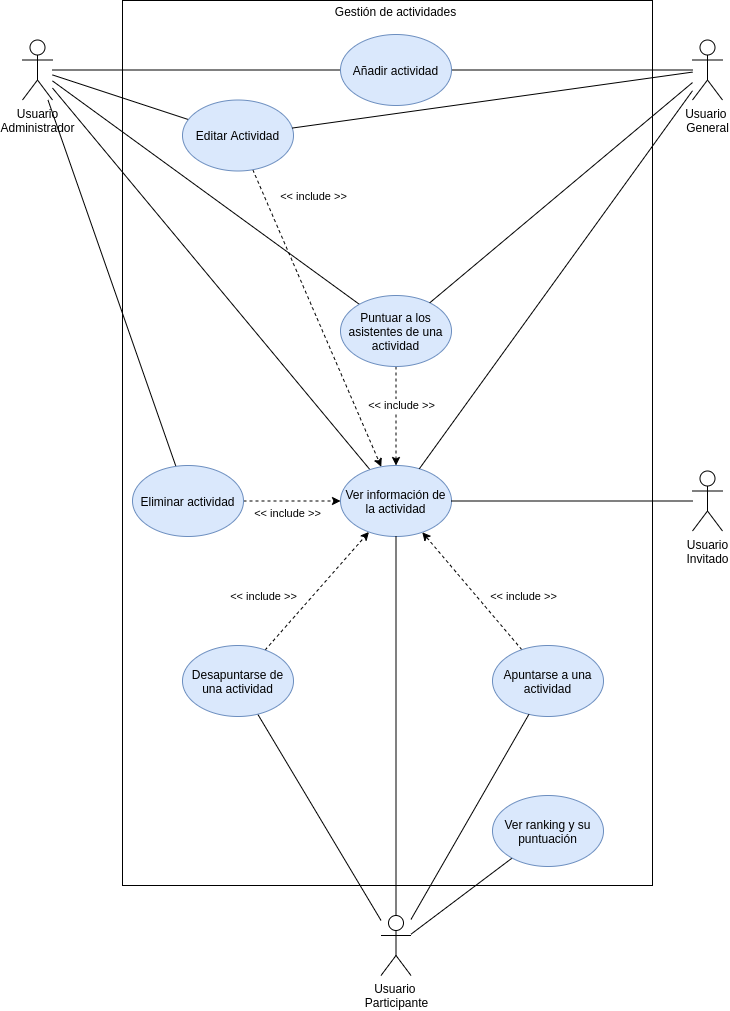
\includegraphics[width=1\linewidth]{diseno/sistema/CU/actividades.png}
    \caption{Diagrama de casos de uso referente a la gestión de actividades}
    \label{fig:cu_actividades}
\end{figure}

\begin{table}[h!]
    \centering
    \resizebox{\textwidth}{!}{
        \begin{tabular}{|l|l|l|l|} 
        \hline
        \rowcolor[rgb]{0.886,0.886,0.886} \textbf{Caso de uso} & \multicolumn{2}{l|}{Puntuar a los asistentes de una actividad} & CU\_06                                                                   \\ 
        \hline
        \textbf{Actores}                                       & \multicolumn{3}{l|}{ACT\_1, ACT\_2}                                                                                                       \\ 
        \hline
        \textbf{Tipo}                                          & \multicolumn{3}{l|}{Primario}                                                                                                             \\ 
        \hline
        \textbf{Referencias}                                   &                      & \multicolumn{2}{l|}{}                                                                                              \\ 
        \hline
        \textbf{Precondición}                                  & \multicolumn{3}{l|}{Se conoce la información de la actividad}                                                                             \\ 
        \hline
        \textbf{Poscondición}                                  & \multicolumn{3}{l|}{}                                                                                                                     \\ 
        \hline
        \textbf{Autor}                                         & Pablo Cordero Romero & \textbf{Versión}                        & 1.0                                                                      \\ 
        \hline
        \multicolumn{4}{l}{}                                                                                                                                                                               \\ 
        \hline
        \multicolumn{4}{|l|}{{\cellcolor[rgb]{0.886,0.886,0.886}}\textbf{Propósito}}                                                                                                                       \\ 
        \hline
        \multicolumn{4}{|l|}{Permitir modificar la puntuación de un usuario en la actividad~~~~~~~~~~~~~~~~~~ }                                                                                            \\ 
        \hline
        \multicolumn{4}{l}{}                                                                                                                                                                               \\ 
        \hline
        \multicolumn{4}{|l|}{{\cellcolor[rgb]{0.886,0.886,0.886}}\textbf{Resumen}}                                                                                                                         \\ 
        \hline
        \multicolumn{4}{|l|}{\begin{tabular}[c]{@{}l@{}}Se modifica la puntuación de un usuario en una actividad concreta,\\modificando a su misma vez todo los referente a los rankings.\end{tabular}}    \\
        \hline
        \end{tabular}
    }
    \caption{Caso de uso 6: Puntuar a los asistentes de una actividad}
    \label{fig:cu_actividades_puntuacion}
\end{table}

\begin{table}[h!]
    \centering
    \resizebox{\textwidth}{!}{
        \begin{tabular}{|l|l|l|l|} 
        \hline
        \multicolumn{4}{|l|}{{\cellcolor[rgb]{0.886,0.886,0.886}}\textbf{Curso Normal (básico) de eventos}}                                                                                                                                                                        \\ 
        \hline
        \multicolumn{2}{|l|}{\textit{\textbf{Actor}}}                                                                                & \multicolumn{2}{l|}{\textit{\textbf{Sistema}}}                                                                                              \\ 
        \hline
        1 & \begin{tabular}[c]{@{}l@{}}El usuario envía la puntuación de\\los diferentes participantes de la\\actividad\end{tabular} & 2 & \begin{tabular}[c]{@{}l@{}}El sistema almacena la puntuación de \\los participantes de la actividad\end{tabular}                        \\ 
        \hline
        &                                                                                                                          & 3 & \begin{tabular}[c]{@{}l@{}}El sistema modifica la información\\referente al ranking, en función al \\cambio de puntuación\end{tabular}  \\ 
        \hline
        4 & \begin{tabular}[c]{@{}l@{}}El usuario recibe la confirmación\\de que se ha realizado\\correctamente\end{tabular}         &   &                                                                                                                                         \\
        \hline
        \end{tabular}
    }
    \caption{Curso de eventos del caso de uso 6}
\end{table}